% !TeX root = ../main.tex

\chapter{多租户性能隔离的闪存资源池化系统设计}

本章介绍本研究提出的多租户性能隔离的闪存资源池化系统设计。
\autoref{sec:design-overview}是对该系统各组件的功能和每一租户获取、访问资源的流程概述。
为了提供没有读写干扰的SSD访问尾延迟,\autoref{sec:design-array}介绍了本系统通过将SSD的访问时间窗口划分为独立的纯读和纯写窗口,避免

\section{系统总述}
\label{sec:design-overview}

如\autoref{fig:design-overview}所示,本系统主要由控制器、客户端和存储单元组成。
其中,控制器负责管理存储单元,并根据租户的需求用尽可能经济的方式为其分配存储空间。
为了避免存储空间的碎片化,控制器以\textit{块}为单位管理存储空间,例如10GB为一个块。
客户端位于租户的虚拟机上,它负责与控制器沟通,并代替租户进行存储资源访问。
存储单元可能是一块SSD或多块SSD组成的存储阵列(~\autoref{sec:design-array}),不同的存储单元可以提供不同的SLA保证,也有不同的开销。
例如,一个存储单元可能用3块SSD的冗余提供99\%分位数的尾延迟保证,而另一个存储单元可能仅能提供90\%的保证,但只需要花费一块SSD。

\begin{figure}[h]
  \centering
  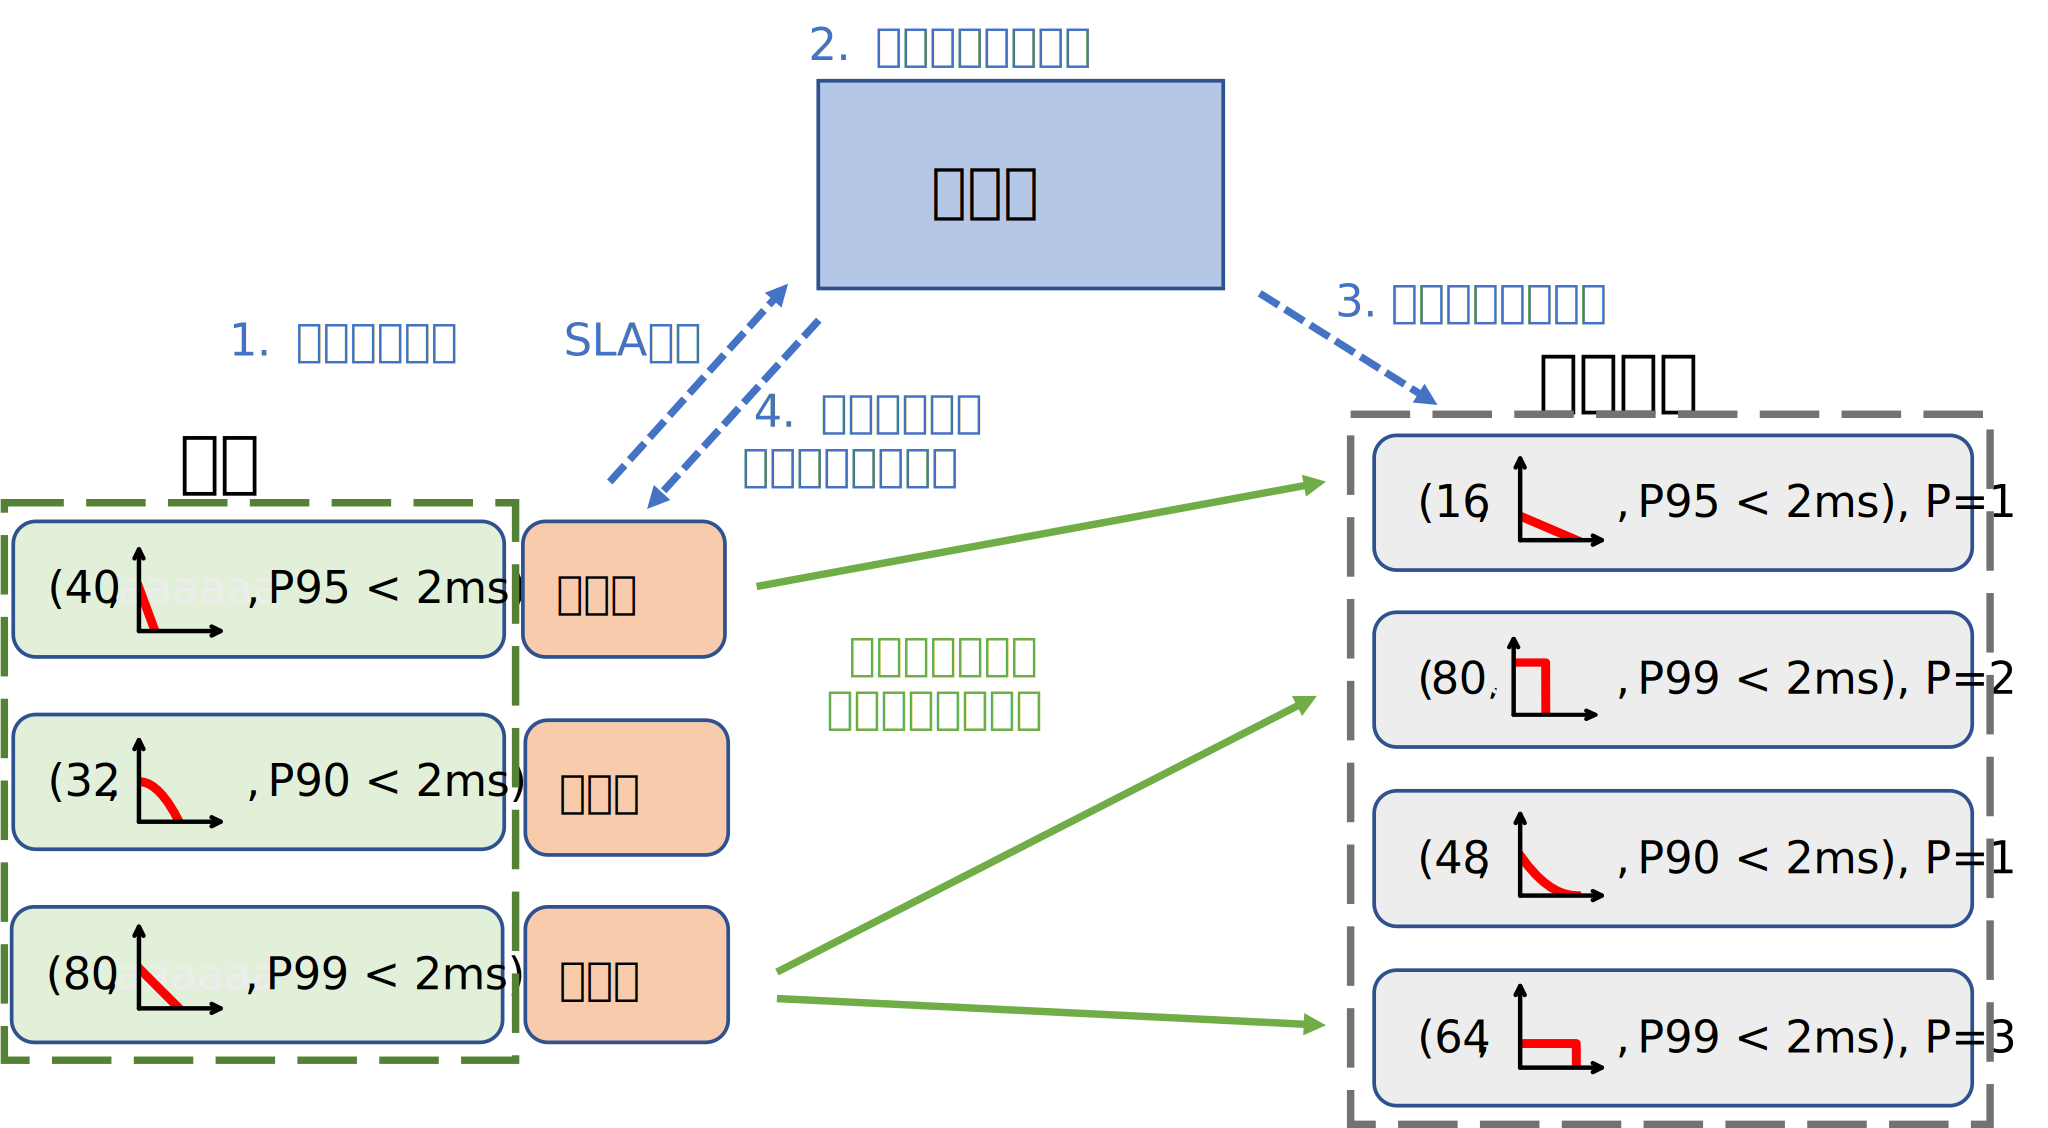
\includegraphics[width=0.8\textwidth]{thesis-design.pdf}
  \caption{
      本系统的总体概述。
      图中蓝色虚线标示的是新租户进入本系统时的控制路径,
      绿色实线标示的是系统中的租户访问存储单元时的数据路径。
      }
  \label{fig:design-overview}
\end{figure}

在本系统中,每个租户的资源需求和每个存储单元能提供的服务能力均以$(C, S, T)$这一三元组定义。
其中,$C$表示存储空间(Capacity),例如40个块;
$S$表示SLA曲线(SLA Curve);
$T$表示尾延迟要求(Tail latency),例如延迟的99\%分位数小于2ms($P99 < 2ms$)。 
由于存储单元的异构性,每个存储单元还有自身的开销$P$。

本系统的控制路径由\autoref{fig:design-overview}中的蓝色虚线表示。
当一个用户加入系统时,他首先通过客户端将自己的资源需求以以上三元组的形式发送给控制器。
控制器以块为单位管理用户的存储需求。
由于每个用户的各个块之间是条带化的\cite{patterson1988case},因此SLA曲线也可以平均分配到每个块上。
根据\autoref{sec:design-allocation}中提出的启发式数据分布算法,控制器优先将尽可能多的块放于已启用的存储单元上。
若已启用的存储单元不足以容纳用户的资源需求,则根据存储单元的开销$P$选择最经济的方式存放剩余的存储需求。
此时若有需要,控制器还需要负责建立新的存储单元(\autoref{sec:design-array})。
在控制器确定该用户的数据分布后,他将该租户的存储空间中每个块与对应的存储单元及存储单元中该块的起始地址的映射发送给租户服务器上的客户端。

\autoref{fig:design-overview}中的绿色实线表示的是本系统的数据路径。
当租户需要访问其所拥有的存储空间时,客户端根据该映射选择合适的存储单元,并将租户存储空间内的逻辑地址转换为存储单元的逻辑地址,从而代替租户访问存储单元。
客户端根据租户的SLA曲线对租户的读写速率进行限制,从而保证租户得到自身的SLA保证。
该客户端可以实现在软件的块设备层~\cite{linuxblock},也可以在智能网卡通过硬件实现~\cite{bluefield}。

\section{无读写干扰的SSD阵列}
\label{sec:design-array}

\subsection{分离的读写时间窗口}
\label{sec:design-array-isorw}

我们的观察:尽可能batch写。上图分析。

介绍设计。

\subsection{读写窗口协调的冗余磁盘阵列}
\label{sec:design-array-composition}

为何一个盘不行?async operations:必须选择大的时间窗口。

组成阵列:利用冗余,协调窗口。

\section{满足SLA要求的数据分布算法}
\label{sec:design-allocation}

并非所有都需要极高的SLA保证:根据SLA需求选择合适的组合。

\subsection{SLA曲线及其运算}
\label{sec:design-allocation-sla-arithmetic}

加法、减法。

\subsection{多租户数据分布算法}
\label{sec:design-allocation-algo}

\begin{algorithm}[h]
  \SetAlgoLined
  \KwData{this text}
  \KwResult{how to write algorithm with \LaTeX2e }

  initialization\;
  \While{not at end of this document}{
    read current\;
    \eIf{understand}{
      go to next section\;
      current section becomes this one\;
    }{
      go back to the beginning of current section\;
    }
  }
  \caption{算法示例1}
  \label{algo:algorithm1}
\end{algorithm}